\chapter{RANSAC: algoritmo de consenso}
En esta sección estudiaremos otro de los algoritmos más utilizados para la alineación de dos nubes de puntos. Se trata del algoritmo \textit{Random Sample Consensus} (RANSAC). El método ICP que acabamos de ver podríamos decir que es específico para la solución de nuestro problema, es decir, no se utiliza más allá de la situación en la que lo hemos estudiado. Por su parte, el algoritmo RANSAC es más genérico y utilizado en otras tareas diferentes. Su finalidad es la de ajustar parámetros de un modelo matemático que viene determinado por un conjunto de observaciones. Nosotros lo utilizaremos para la detección de superficies planas en nuestros modelos que a su vez las utilizaremos para la obtención de sus puntos intersección. Esos puntos que podríamos considerarlos como clave, siguiendo la nomenclatura utilizada, serán la base para el alineado. Destacar que es considerado un algoritmo robusto incluso bajo la existencia de gran cantidad de valores atípicos y que sigue un paradigma de hipótesis-y-prueba.

\section{Algoritmo}
Este algoritmo fue propuesto por A. Fischler y Robert C. Bolles en \cite{fischler1981random}. Este será el artículo que seguiremos como referencia en lo que respecta a la explicación matemática de la veracidad del método. Como hemos dicho en la introducción, podemos considerar que es un algoritmo del tipo hipótesis-y-prueba. A diferencia de otros algoritmos, no tiene en cuenta todo el conjunto, sino que toma el menor número posible de puntos necesarios para ajustar el modelo y comprueba si efectivamente esos puntos determinan el modelo que queremos. En nuestro caso, el modelo que deseamos obtener es un plano.\\

El algoritmo consta de las siguientes etapas:
\begin{enumerate}
\item Tomar de manera aleatoria el mínimo número de puntos necesarios que define el modelo.
\item Con una tolerancia $ \varepsilon$, contar el número de puntos que distan del modelo definido en el punto anterior.
\item Repetir 1 y 2 un total de $ N $ veces y quedarse con el que contenga una mayor cantidad de puntos.
\end{enumerate}

De este modo, podemos considerar que el algoritmo necesita, por ahora, tres parámetros. El primero de ellos, el mínimo número de puntos para definir el modelo. Por ejemplo, si queremos obtener una recta debemos tomar 2 puntos mientras que si queremos obtener un plano debemos coger 3. También tenemos que decidir una tolerancia $ \varepsilon $ que depende, en cierto modo, de la nube de puntos que tenemos entre manos y del resultado final que queremos. Finalmente, hay que decidir un $ N $ que determina el número de veces que repetimos el proceso. Su cálculo se explicará en siguientes secciones pero destacamos ahora que debe de ser lo suficientemente grande para asegurar que este proceso aleatorio conseguirá nuestro objetivo. \\

Antes de continuar, veamos un ejemplo sencillo en dos dimensiones donde explicaremos cómo funciona este procedimiento. Supongamos que tenemos la nube de la figura \ref{fig:ejransac0}. \\

\begin{figure}[h!]
	\centering
	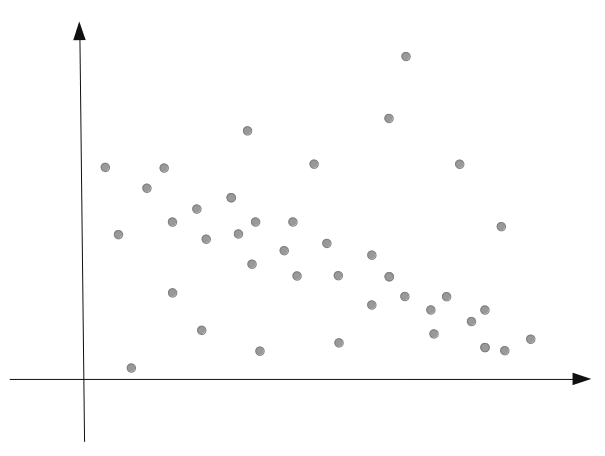
\includegraphics[width=0.5\linewidth]{imagenes/Ej-RANSAC/ejRANSAC_0}
	\caption{Nube de puntos.}
	\label{fig:ejransac0}
\end{figure}

Queremos aplicarle el algoritmo RANSAC para obtener una recta dentro de ella. Para ello, primero cogemos dos puntos aleatorios del modelo, calculamos al recta que pasa por ellos, y obtenemos los puntos que distan de la misma una distancia menor que $ \varepsilon $. Supongamos que la situación es la que se muestra en la figura \ref{fig:RNASAC-s1}. \\

\begin{figure}[h!]
	\begin{minipage}[b]{0.5\textwidth}
		\centering
		%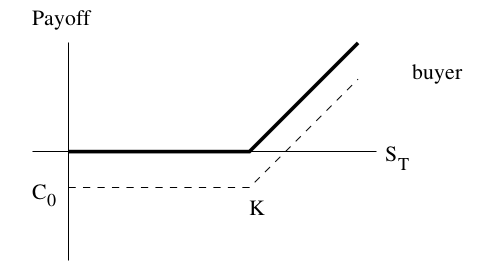
\includegraphics[width=1\linewidth]{Buyer_call} 
		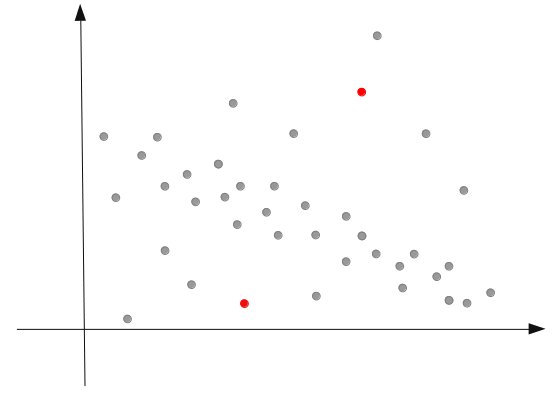
\includegraphics[width=1\linewidth]{Ej-RANSAC/ejRANSAC_10} 
		\caption*{Selección de puntos.}
		%\label{fig:subim1}
	\end{minipage}
\begin{minipage}[b]{0.5\textwidth}
	\centering
	%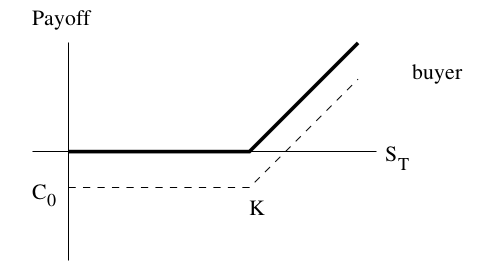
\includegraphics[width=1\linewidth]{Buyer_call} 
	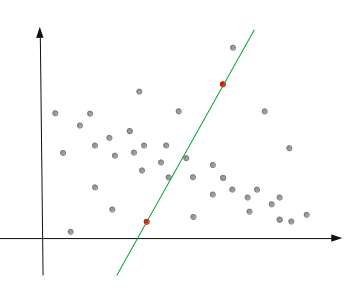
\includegraphics[width=1\linewidth]{Ej-RANSAC/ejRANSAC_11} 
	\caption*{Construcción de la recta}
	%\label{fig:subim1}
\end{minipage}
\begin{center}
	\begin{minipage}[b]{0.5\textwidth}
	\centering
	%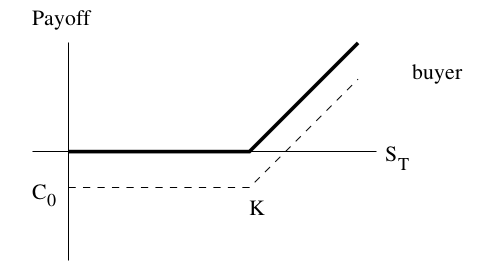
\includegraphics[width=1\linewidth]{Buyer_call} 
	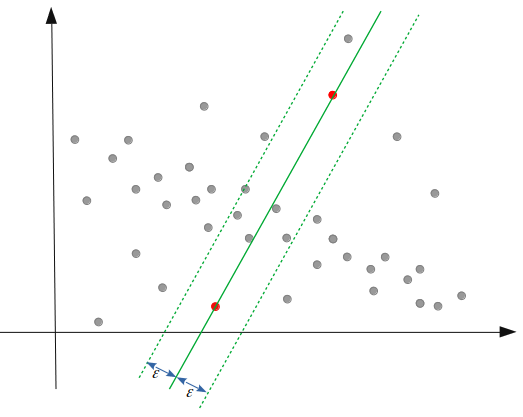
\includegraphics[width=1\linewidth]{Ej-RANSAC/ejRANSAC_12} 
	\caption*{Vemos la bondad del modelo.}
	%\label{fig:subim1}
\end{minipage}
\end{center}
	\caption{Primer paso del algoritmo RANSAC.}
	\label{fig:RNASAC-s1}
\end{figure}

Si contamos el número de puntos que se ajustan al modelo, vemos que hay un total de 8. Repetimos el proceso y, en una iteración determinada, se obtiene el modelo de la figura \ref{fig:RNASAC-s2}.\\

\begin{figure}[h!]
	\begin{minipage}[b]{0.5\textwidth}
		\centering
		%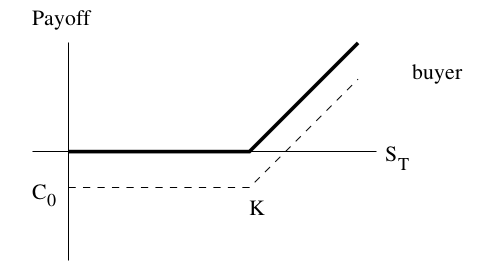
\includegraphics[width=1\linewidth]{Buyer_call} 
		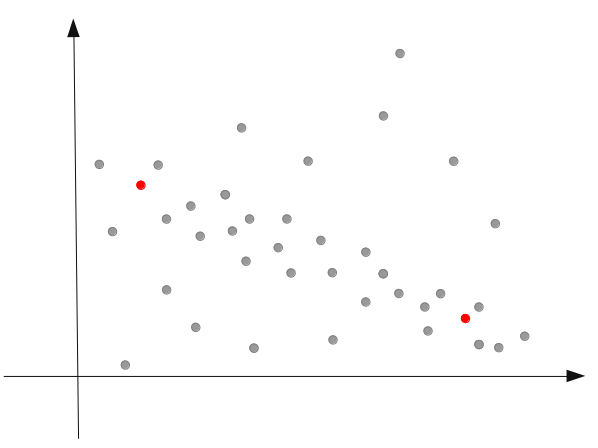
\includegraphics[width=1\linewidth]{Ej-RANSAC/ejRANSAC_20} 
		\caption*{Selección de puntos.}
		%\label{fig:subim1}
	\end{minipage}
	\begin{minipage}[b]{0.5\textwidth}
		\centering
		%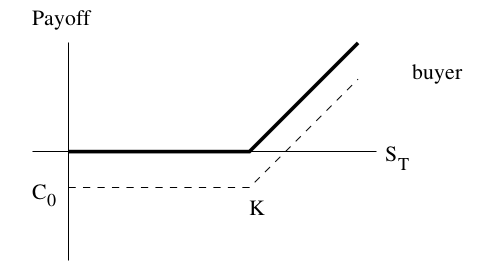
\includegraphics[width=1\linewidth]{Buyer_call} 
		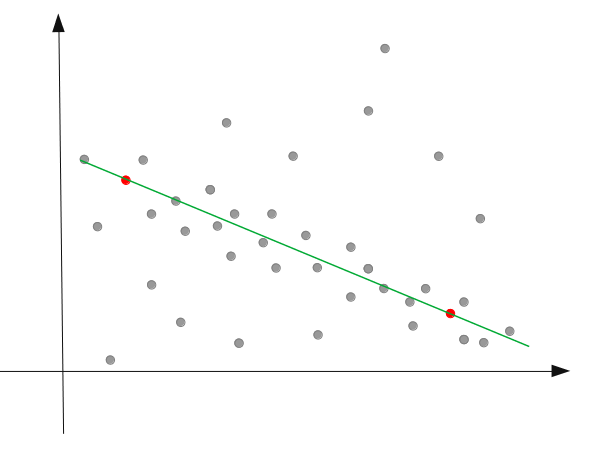
\includegraphics[width=1\linewidth]{Ej-RANSAC/ejRANSAC_21} 
		\caption*{Construcción de la recta}
		%\label{fig:subim1}
	\end{minipage}
	\begin{center}
		\begin{minipage}[b]{0.5\textwidth}
		\centering
		%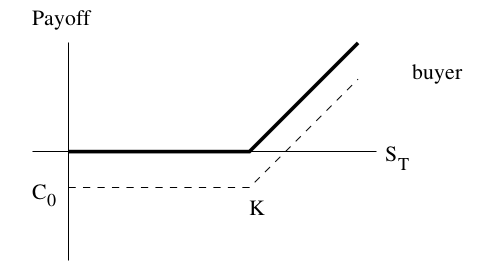
\includegraphics[width=1\linewidth]{Buyer_call} 
		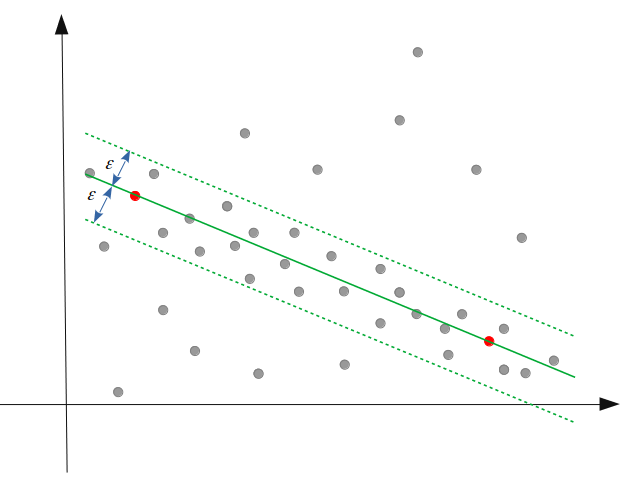
\includegraphics[width=1\linewidth]{Ej-RANSAC/ejRANSAC_22} 
		\caption*{Vemos la bondad del modelo.}
		%\label{fig:subim1}
	\end{minipage}
	\end{center}
	\caption{Paso del algoritmo RANSAC.}
	\label{fig:RNASAC-s2}
\end{figure}
Ene esta ocasión, un total de 27 puntos se ajustan al modelo. Si no se detectara en el resto de iteraciones un ajuste mejor, este sería el modelo que nos devolvería al algoritmo. \\

\section{Número de iteraciones}
Uno de los puntos clave del algoritmo es asegurarse de que el número de iteraciones $ N $ sea lo suficientemente grande para obtener puntos que ajusten correctamente el modelo que queremos. De este modo, sea $ p $ la probabilidad que al menos uno de los conjuntos tomados no contiene valores atípicos y $ 1-p $ de que todos los conjuntos contienen al menos un valor atípico. Notamos por $ u $, a la probabilidad de que un valor sea correcto y, por lo tanto, $ v = 1 - u $ es la probabilidad de ser un valor atípico. Sea $ m $ el número de puntos mínimo para definir el modelo: dos para una recta, tres para un plano, $ \dots $. Así, la probabilidad de escoger todos los puntos correctos en una iteración es $ u^m $ y la de escoger alguno incorrecto es $ 1-u^m $. Si hacemos un total de $ N $ iteraciones, la probabilidad de escoger siempre un valor atípico es $ (1-u^m)^N $. Pero esto no es más que
\[
1-p = (1-u^m)^N.
\]
Si despejamos el valor de $ N $,
\begin{equation}
N = \frac{\log(1-p)}{\log(1-u^m)} = \frac{\log(1-p)}{\log(1-(1-v)^m)}.
\end{equation}
El valor obtenido no tiene que ser obligatoriamente un número natural por lo que se toma el primero entero que supere o iguale dicho valor. La probabilidad $ p $ es entrada del algoritmo y debe ser elevado. También $ u $ (o $ v $) son parámetros que se eligen y que dependerán en cierto modo, del modelo con el que se está trabajando. La tabla \ref{table:RANSAcvalues} recoge diferentes valores de $ N $ en función de $ p $, $ v $ y $ m $.
% Please add the following required packages to your document preamble:
% \usepackage{multirow}
% Please add the following required packages to your document preamble:
% \usepackage{multirow}
% Please add the following required packages to your document preamble:
% \usepackage{multirow}
% Please add the following required packages to your document preamble:
% \usepackage{multirow}
% Please add the following required packages to your document preamble:
% \usepackage{multirow}
\begin{table}[]
	\centering
	\begin{tabular}{l|l|c|c|c|c|}
		\cline{2-6}
		& \multirow{2}{*}{$ m $} & \multicolumn{4}{c|}{$ v $}                                                                                     \\ \cline{3-6} 
		&                    & \multicolumn{1}{l|}{0.05} & \multicolumn{1}{l|}{0.2} & \multicolumn{1}{l|}{0.5} & \multicolumn{1}{l|}{0.8} \\ \hline
		\multicolumn{1}{|l|}{\multirow{2}{*}{$ p = 0.99 $}} & 2                  & 2                         & 5                        & 17                       & 113                      \\ \cline{2-6} 
		\multicolumn{1}{|l|}{}                          & 3                  & 3                         & 7                        & 35                       & 574                      \\ \hline
		\multicolumn{1}{|l|}{\multirow{2}{*}{$ p = 0.9 $}}  & 2                  & 1                         & 3                        & 9                        & 57                       \\ \cline{2-6} 
		\multicolumn{1}{|l|}{}                          & 3                  & 2                         & 4                        & 18                       & 287                      \\ \hline
		\multicolumn{1}{|l|}{\multirow{2}{*}{$ p = 0.8 $}}  & 2                  & 1                         & 2                        & 6                        & 40                       \\ \cline{2-6} 
		\multicolumn{1}{|l|}{}                          & 3                  & 1                         & 3                        & 13                       & 201                      \\ \hline
	\end{tabular}
\caption{Número de iteraciones para diferentes valores de $ p $ (probabilidad), $ m $ (número de puntos para definir el modelo: 2 recta y 3 plano) y $ v $ probabilidad de ser un valor atípico.}
\label{table:RANSAcvalues}
\end{table}


\section{Ejemplos sencillos}
En esta sección, veremos cómo actúa al algoritmo en dos ejemplos concretos: el del pie y en el de la torre. En ambos casos usaremos los modelos simplificados tal y como hemos visto en la sección \ref{varNormal}. Esto no debería de ser una restricción ya que la densidad total del modelo no varía y los planos se mantienen. Para cada, utilizaremos diferente valores de los parámetros y veremos cómo de buenos son los resultados obtenidos. Al ser modelos en los que buscamos planos el valor de $ m $ es 3. Destacamos que para el cálculo de la distancia entre el modelo y cada punto se ha hecho mediante la función distancia con signo (en valor absoluto).

\subsection{Pie}
Se ha tomado como nivel de tolerancia $ \varepsilon = 0.05 $ ya que ese valor depende sobre todo del modelo que estamos trabajando. El modelo consta de un total de $ 34.120 $ puntos. En la tabla \ref{table:RANSACpieTable} y en la figura \ref{fig:RANSACpie} están los resultados que nos proporciona. \\

\begin{figure}[h!]
	\begin{minipage}[b]{0.5\textwidth}
		\centering
		%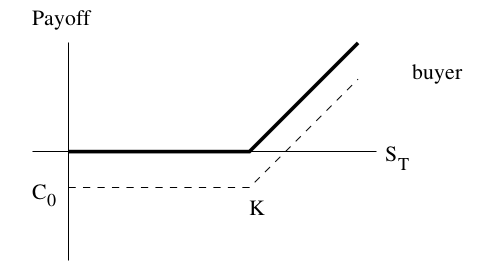
\includegraphics[width=1\linewidth]{Buyer_call} 
		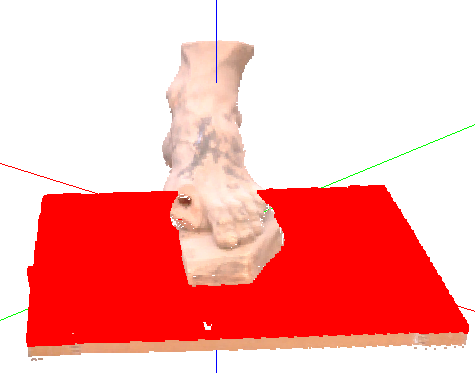
\includegraphics[width=0.8\linewidth]{Ej-RANSAC/pie_0-5_0-4} 
		\caption*{(a)}
		%\label{fig:subim1}
	\end{minipage}
	\begin{minipage}[b]{0.5\textwidth}
		\centering
		%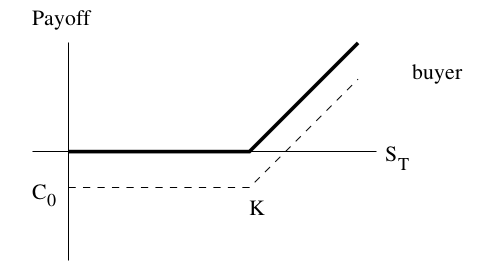
\includegraphics[width=1\linewidth]{Buyer_call} 
		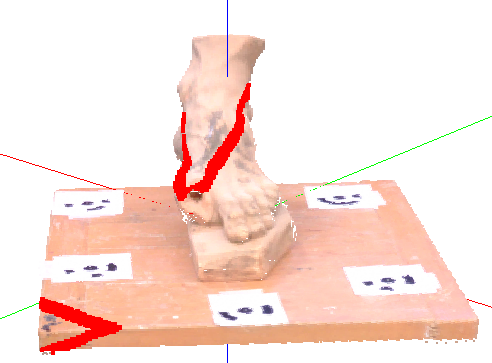
\includegraphics[width=0.8\linewidth]{Ej-RANSAC/pie_0-5_0-3} 
		\caption*{(b)}
		%\label{fig:subim1}
	\end{minipage}
	\begin{minipage}[b]{0.5\textwidth}
		\centering
		%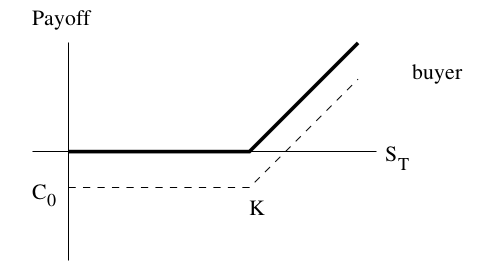
\includegraphics[width=1\linewidth]{Buyer_call} 
		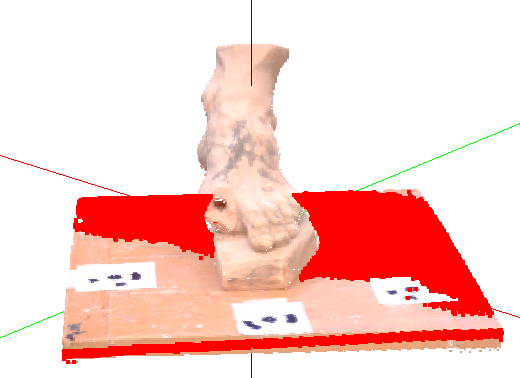
\includegraphics[width=0.8\linewidth]{Ej-RANSAC/pie_0-7_0-3} 
		\caption*{(c)}
		%\label{fig:subim1}
	\end{minipage}
	\begin{minipage}[b]{0.5\textwidth}
		\centering
		%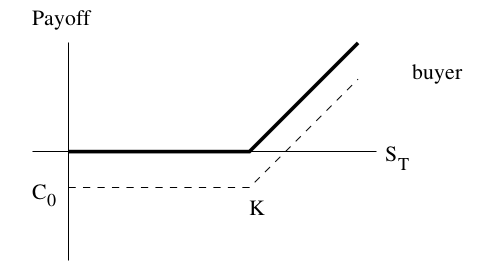
\includegraphics[width=1\linewidth]{Buyer_call} 
		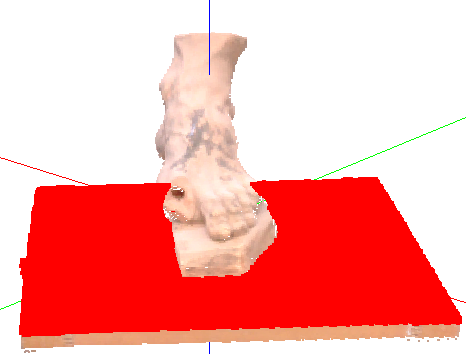
\includegraphics[width=0.8\linewidth]{Ej-RANSAC/pie_0-9_0-3} 
		\caption*{(d)}
		%\label{fig:subim1}
	\end{minipage}		
	\begin{minipage}[b]{0.5\textwidth}
		\centering
		%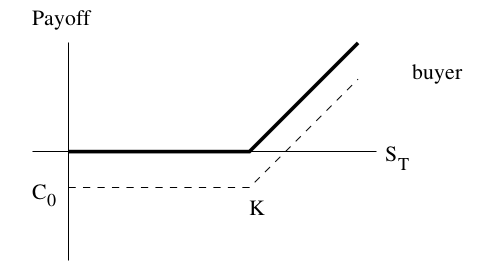
\includegraphics[width=1\linewidth]{Buyer_call} 
		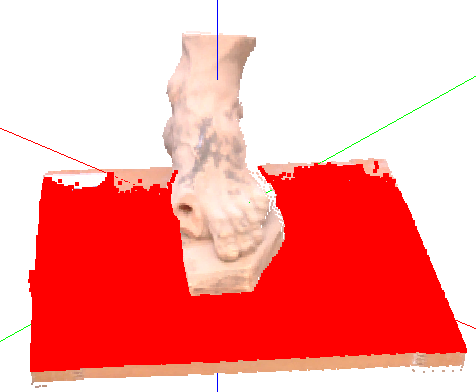
\includegraphics[width=0.8\linewidth]{Ej-RANSAC/pie_0-9_0-5} 
		\caption*{(e)}
		%\label{fig:subim1}
	\end{minipage}
	\begin{minipage}[b]{0.5\textwidth}
		\centering
		%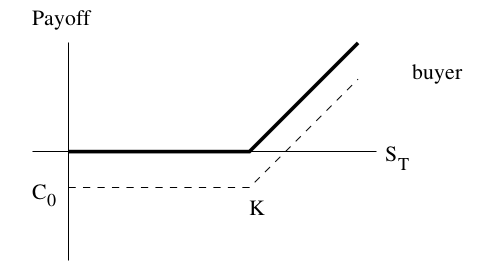
\includegraphics[width=1\linewidth]{Buyer_call} 
		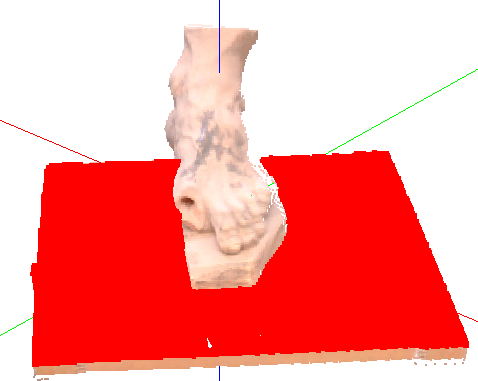
\includegraphics[width=0.8\linewidth]{Ej-RANSAC/pie_0-9_0-7} 
		\caption*{(f)}
		%\label{fig:subim1}
	\end{minipage}	
	
	\caption{Resultados de aplicar RANSAC en el ejemplo del pie para diferentes parámetros (ver tabla \ref{table:RANSACpieTable}). }
	\label{fig:RANSACpie}
\end{figure}

\begin{table}[h!]
	\centering
	\begin{tabular}{| c | c | c || c | c |} 
		\hline
		Prueba & $ p $ & $ v $ & Tiempo (seg.) & Iteraciones \\
		\hline
		(a) & 0.5 & 0.4 & 0.0521721 & 3 \\		
		(b) & 0.5 & 0.3 & 0.0260945 & 2  \\	
		(c) & 0.7 & 0.3 & 0.055964 &  3 \\
		(d) & 0.9 & 0.3 & 0.116656 & 6\\
		(e) & 0.9 & 0.5 & 0.356769 & 18\\
		(f) & 0.9 & 0.7 & 1.7125 & 85\\
		\hline
	\end{tabular}
	\caption{Resultados de aplicar el algoritmo RANSAC una vez a una toma del pie. La primera columna identifica la prueba (ver figura \ref{fig:RANSACpie}), la segunda y tercera los valores de $ p $ y $ v $ escogidos y las dos últimas el tiempo empleado en el cálculo del plano y las iteraciones que se han realizado.}
	\label{table:RANSACpieTable}
\end{table}

Vemos que al ser un proceso aleatorio los resultados que se han obtenido son dispares pero en este caso, en un número ``bajo'' de iteraciones hemos visto que es capaz de detectar el plano que contiene el modelo.

\subsection{Torre}
Realizamos diferentes pruebas con nuestro modelo de la torre que consta de $ 431\,254 $ puntos. En esta ocasión se ha optado por una tolerancia de $ \varepsilon = 0.03 $. Los resultados se recogen en la tabla \ref{table:RANSACtorreTable} y en la figura \ref{fig:RANSACtorre}. \\

\begin{figure}[h!]
	\begin{minipage}[b]{0.5\textwidth}
		\centering
		%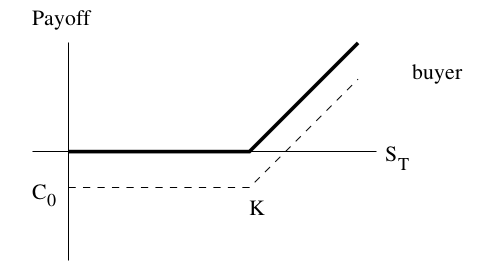
\includegraphics[width=1\linewidth]{Buyer_call} 
		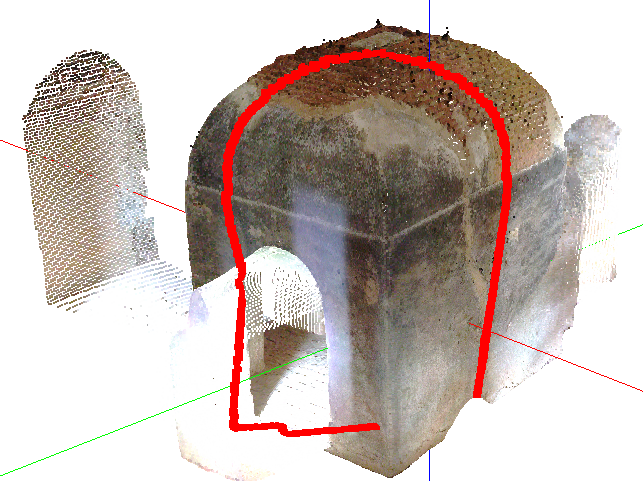
\includegraphics[width=0.8\linewidth]{Ej-RANSAC/torre_0-5_0-4} 
		\caption*{(a2)}
		%\label{fig:subim1}
	\end{minipage}
	\begin{minipage}[b]{0.5\textwidth}
		\centering
		%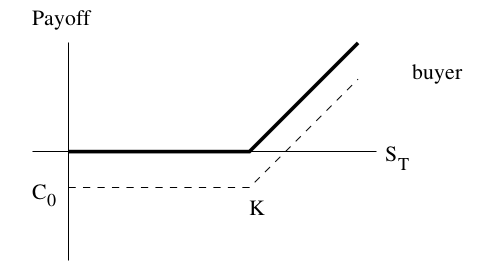
\includegraphics[width=1\linewidth]{Buyer_call} 
		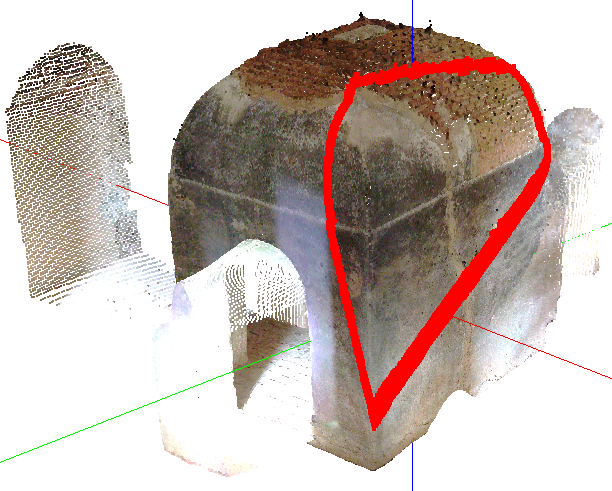
\includegraphics[width=0.8\linewidth]{Ej-RANSAC/torre_0-7_0-4} 
		\caption*{(b2)}
		%\label{fig:subim1}
	\end{minipage}
	\begin{minipage}[b]{0.5\textwidth}
		\centering
		%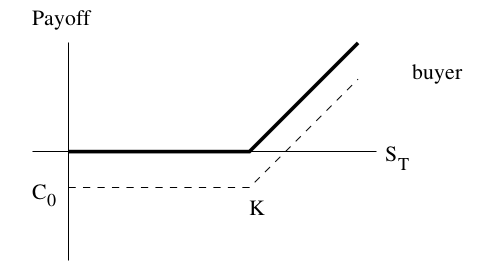
\includegraphics[width=1\linewidth]{Buyer_call} 
		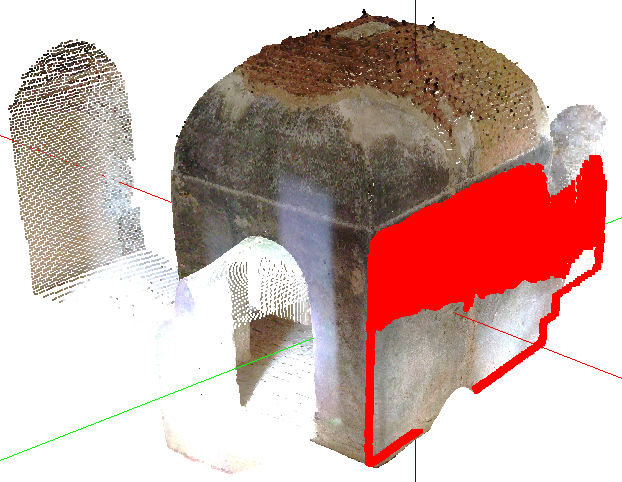
\includegraphics[width=0.8\linewidth]{Ej-RANSAC/torre_0-7_0-6} 
		\caption*{(c2)}
		%\label{fig:subim1}
	\end{minipage}
	\begin{minipage}[b]{0.5\textwidth}
		\centering
		%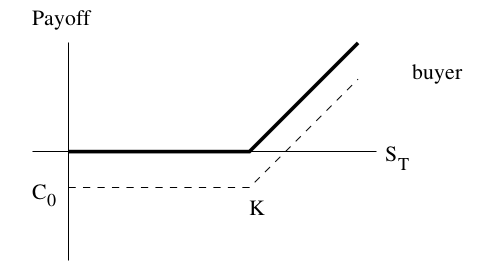
\includegraphics[width=1\linewidth]{Buyer_call} 
		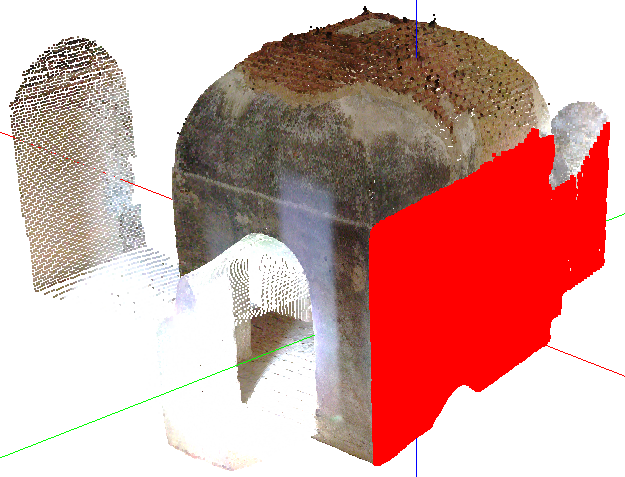
\includegraphics[width=0.8\linewidth]{Ej-RANSAC/torre_0-8_0-6} 
		\caption*{(d2)}
		%\label{fig:subim1}
	\end{minipage}		
	\begin{minipage}[b]{0.5\textwidth}
		\centering
		%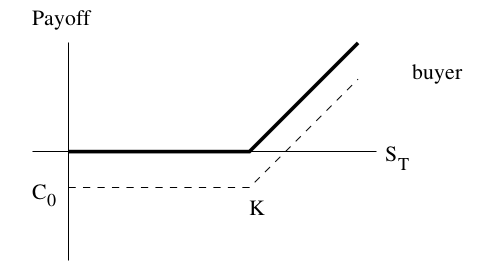
\includegraphics[width=1\linewidth]{Buyer_call} 
		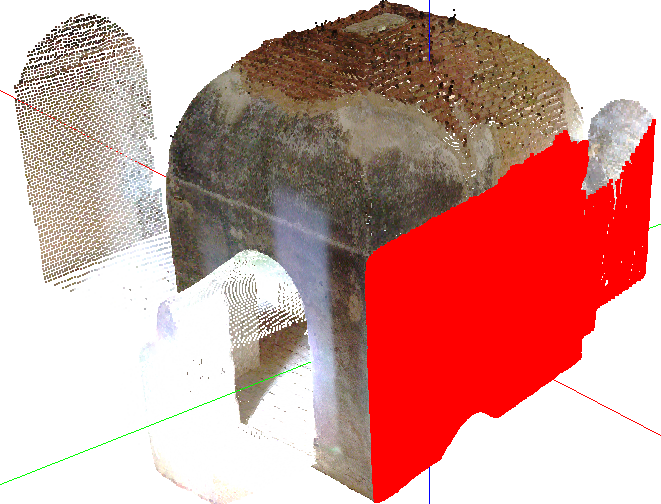
\includegraphics[width=0.8\linewidth]{Ej-RANSAC/torre_0-8_0-7} 
		\caption*{(e2)}
		%\label{fig:subim1}
	\end{minipage}
	\begin{minipage}[b]{0.5\textwidth}
		\centering
		%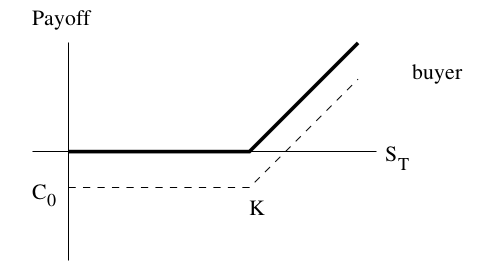
\includegraphics[width=1\linewidth]{Buyer_call} 
		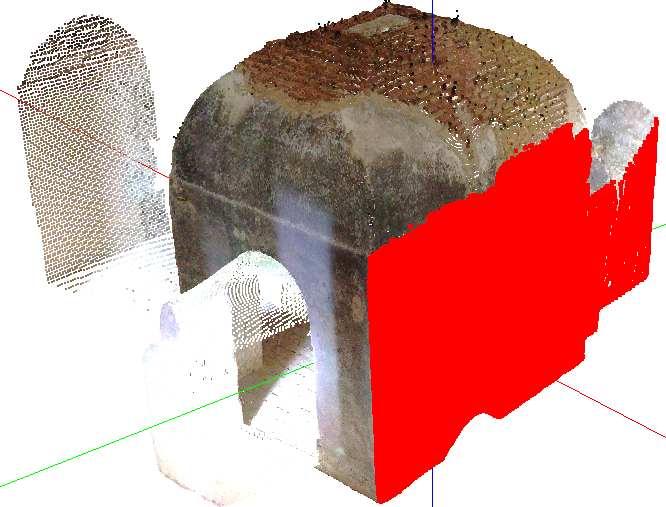
\includegraphics[width=0.8\linewidth]{Ej-RANSAC/torre_0-85_0-8} 
		\caption*{(f2)}
		%\label{fig:subim1}
	\end{minipage}	
	
	\caption{Resultados de aplicar RANSAC en el ejemplo de la torre para diferentes parámetros (ver tabla \ref{table:RANSACtorreTable}). }
	\label{fig:RANSACtorre}
\end{figure}

\begin{table}[h!]
	\centering
	\begin{tabular}{| c | c | c || c | c |} 
		\hline
		Prueba & $ p $ & $ v $ & Tiempo (seg.) & Iteraciones \\
		\hline
		(a2) & 0.5 & 0.4 & 0.484033 & 3 \\		
		(b2) & 0.7 & 0.4 & 0.961606 & 5  \\	
		(c2) & 0.7 & 0.6 & 4.27183 &  19 \\
		(d2) & 0.8 & 0.6 & 5.74916 & 25\\
		(e2) & 0.8 & 0.7 & 14.0042 & 59 \\
		(f2) & 0.85 & 0.8 & 55.9862 & 237\\
		\hline
	\end{tabular}
	\caption{Resultados de aplicar el algoritmo RANSAC una vez a una toma de  la torre. La primera columna identifica la prueba (ver figura \ref{fig:RANSACpie}), la segunda y tercera los valores de $ p $ y $ v $ escogidos y las dos últimas el tiempo empleado en el cálculo del plano y las iteraciones que se han realizado.}
	\label{table:RANSACtorreTable}
\end{table}

Vemos que nuevamente se han podido obtener resultados buenos en relativamente pocas iteraciones.

\section{Cálculo de los puntos de intersección}
En esta sección, vamos a obtener mediante el algoritmo RANSAC un punto que sea intersección de tres planos. Para ello, tomamos el ejemplo de la torre. En primer lugar, veamos cómo calculamos dicha intersección. Lo único que tenemos que hacer, dado un conjunto de puntos que hemos obtenido como plano, es tomar una normal del mismo. Esta normal puede ser, por ejemplo, la misma que hemos usado para el cálculo de las distancias mediante la función distancia con signo que la podemos ir almacenando para evitar su cálculo posterior. Notamos a la normal obtenida para el paso $ i $ como $ N_i = (N_{i1}, N_{i2}, N_{i3}) \in \RR^3$. De este modo, cada punto $ (x,y,z) $ del conjunto debe cumplir la ecuación:
\[
N_{i1} x + N_{i2} y + N_{i3} z = d_i.
\]
Finalmente, solo nos queda calcular $ d _i$, que se puede hacer de manera sencilla sustituyendo el valor de $ (x,y,z) $ por un punto conocido del conjunto obtenido. Hemos calculado la ecuación del plano de una manera sencilla. Ahora solo nos queda calcular la intersección de tres planos. Para ello, tenemos que resolver el sistema para las iteraciones $ i,j,k $:

\[
\left.
\begin{array}{rcl}
&N_{i1}x + N_{i2}y + N_{i3}z  &= d_i \\ 
&N_{j1}x + N_{j2}y + N_{j3}z  &= d_j \\
&N_{k1}x + N_{k2}y + N_{k3}z  &= d_k
\end{array}
\right\}
\]
\[
\big\Updownarrow
\]
\[
\begin{pmatrix}
N_{i1} & N_{i2} & N_{i3}\\
N_{j1} & N_{j2} & N_{j3}\\
N_{k1} & N_{k2} & N_{k3}\\
\end{pmatrix}
\begin{pmatrix}
x\\
y\\
z\\
\end{pmatrix}
=
\begin{pmatrix}
d_i\\
d_j\\
d_k\\
\end{pmatrix}
\]
\[
\big\Updownarrow
\]
\[
A \begin{pmatrix}
x\\
y\\
z\\
\end{pmatrix}
=
\mathit{\mathbf{d}}.
\]

Si el sistema es compatible determinado, lo que significa que la intersección está formada solo por un punto, podemos calcular $ A^{-1} $ y obtenemos el punto de intersección como:
\[
\begin{pmatrix}
x\\
y\\
z\\
\end{pmatrix} = A^{-1}\mathbf{d}.
\]

Veamos este caso en el modelo real. Primero, obtenemos tres planos de la nube de puntos. Usamos el algoritmo con valor $ p = 0.8 $, $ v = 0.8 $ y $ \varepsilon = 0.03 $. Los planos que se han obtenido se muestran en la siguiente figura \ref{fig:RNASACptoInter}. \\
\begin{figure}[h!]
	\begin{minipage}{0.5\textwidth}
		\centering
		%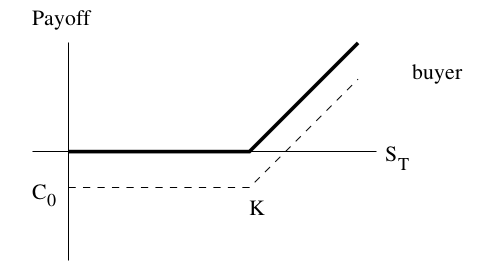
\includegraphics[width=1\linewidth]{Buyer_call} 
		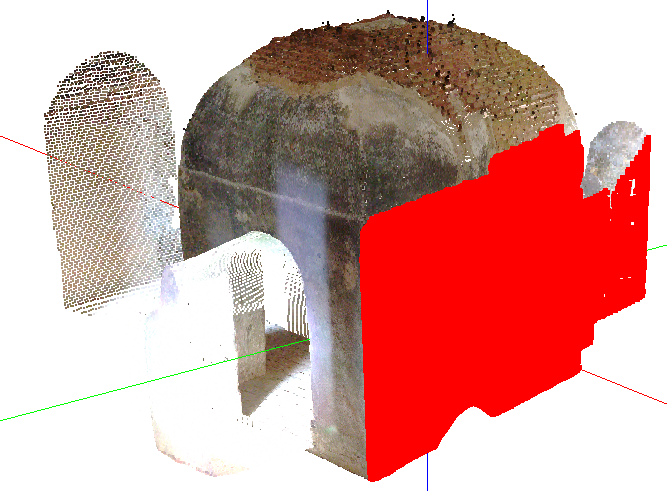
\includegraphics[width=0.8\linewidth]{Ej-RANSAC/torre_1-1} 
		%\label{fig:subim1}
	\end{minipage}
	\begin{minipage}{0.5\textwidth}
		\centering
		%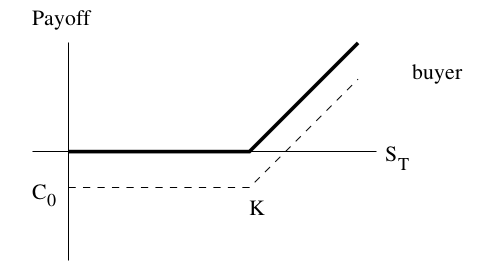
\includegraphics[width=1\linewidth]{Buyer_call} 
		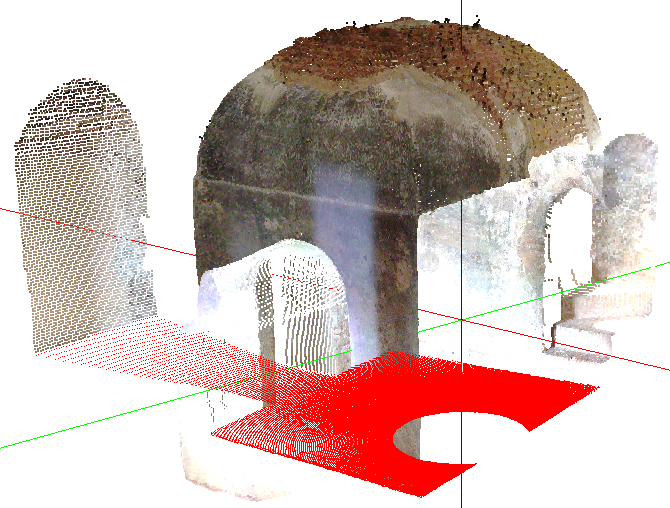
\includegraphics[width=0.8\linewidth]{Ej-RANSAC/torre_1-2} 
		%\label{fig:subim1}
	\end{minipage}
	\begin{center}
		\begin{minipage}{0.5\textwidth}
		\centering
		%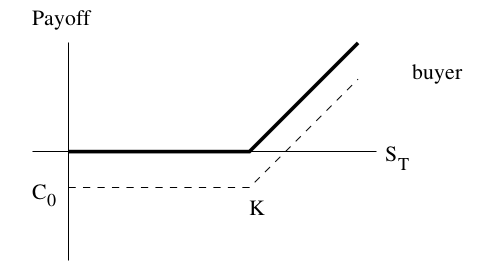
\includegraphics[width=1\linewidth]{Buyer_call} 
		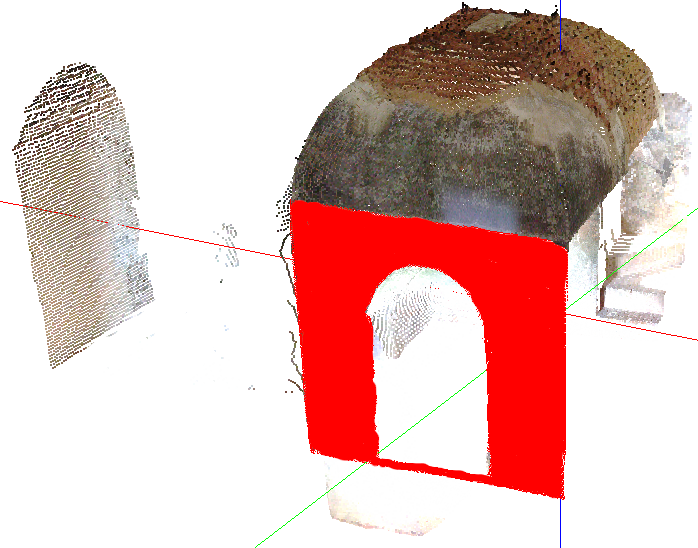
\includegraphics[width=0.8\linewidth]{Ej-RANSAC/torre_1-3} 
		%\label{fig:subim1}
	\end{minipage}
	\end{center}
	\caption{Planos detectados iterativamente en el ejemplo de la torre de las gallinas de la Alhambra. Los parámetros son $ p = 0.8 $, $ v = 0.8 $ y $ \varepsilon = 0.03 $.}
	\label{fig:RNASACptoInter}
\end{figure}

Los valores que se han obtenido han sido los siguientes:
\begin{itemize}
\item $ N_1 = ( 0.987981, 0.154204, 0.0107157) $, $ d_1 = -0.50992 $.
\item $ N_2 = ( -0.0192558, 0.0458887, 0.998761) $, $ d_2 = -1.13957 $.
\item $ N_3 = ( 0.147295, -0.987795, 0.0506549) $, $ d_3 = -1.34888$.
\end{itemize}
Claramente, el sistema que forman es compatible determinado. Si lo resolvemos tal y como se ha explicado anteriormente obtenemos el punto $ (-0.690391, 1.20058, -1.20946) $ que se corresponde con el marcado en la figura \ref{fig:torre1-4}.
\begin{figure}
	\centering
	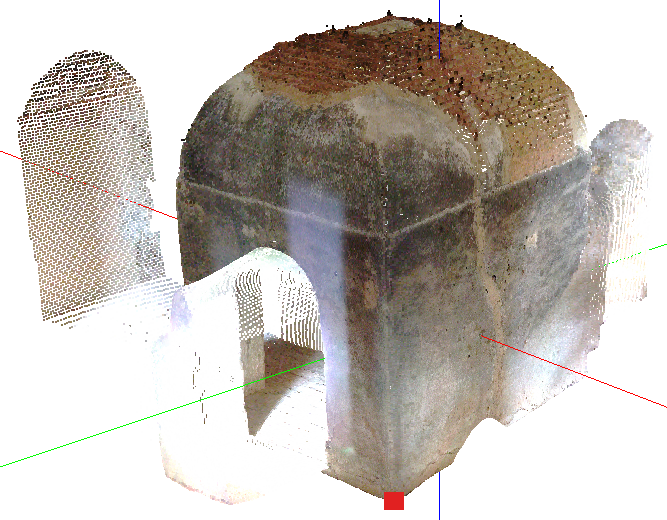
\includegraphics[width=0.4\linewidth]{imagenes/Ej-RANSAC/torre_1-4}
	\caption{Punto de intersección.}
	\label{fig:torre1-4}
\end{figure}


\section{Ejemplo despacho}
El objetivo de esta sección es probar el comportamiento del algoritmo en un ejemplo más complejo y del que podemos obtener un mayor número de planos. En concreto, se trata de dos tomas de un despacho. Destacamos que nuevamente se ha realizado el proceso de simplificado de las mismas con un nivel de 4 y tras este proceso se han obtenido aproximadamente $ 650\,000 $ puntos en cada toma. En la figura \ref{fig:tomasLab} se muestran ambas nubes de puntos. 

\begin{figure}[h!]
	\begin{minipage}[b]{0.5\textwidth}
		\centering
		%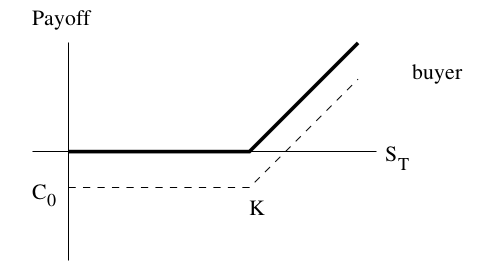
\includegraphics[width=1\linewidth]{Buyer_call} 
		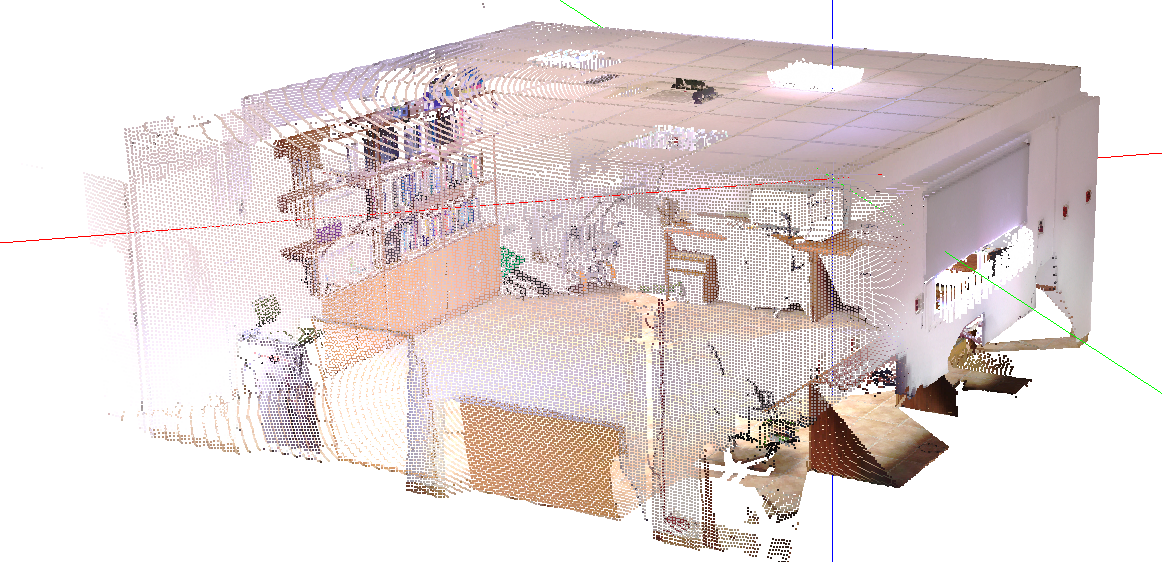
\includegraphics[width=1\linewidth]{lab/LAB0} 
		\caption*{Toma 0.}
		%\label{fig:subim1}
	\end{minipage}
	\begin{minipage}[b]{0.5\textwidth}
		\centering
		%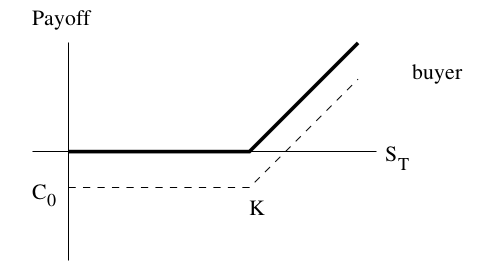
\includegraphics[width=1\linewidth]{Buyer_call} 
		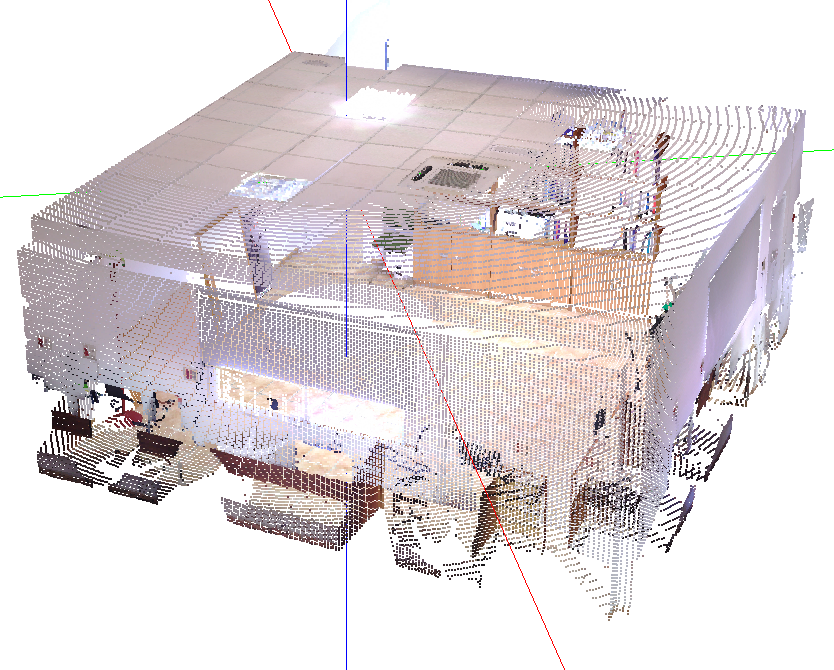
\includegraphics[width=0.8\linewidth]{lab/LAB1} 
		\caption*{Toma 1.}
		%\label{fig:subim1}
	\end{minipage}
	\caption{Tomas del laboratorio.}
	\label{fig:tomasLab}
\end{figure}

En primer lugar, veamos los planos que se obtienen al ejecutar el algoritmo RANSAC en la primera de ellas. Los planos obtenidos se muestran en la figura \ref{fig:planos-lab0}. Posteriormente, en la tabla \ref{table:res-lab0} aparece el tiempo empleado y el número de puntos detectados en cada plano. Finalmente, en la figura \ref{fig:inter0} están los puntos de intersección obtenidos. \\

\begin{figure}[h!]
	\centering
	\begin{minipage}{0.4\textwidth}
		\centering
		%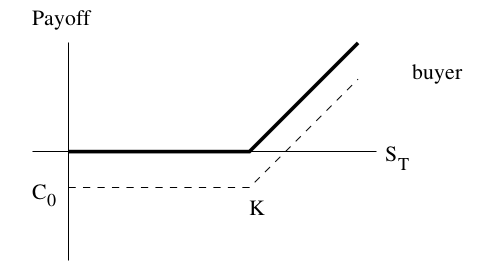
\includegraphics[width=1\linewidth]{Buyer_call} 
		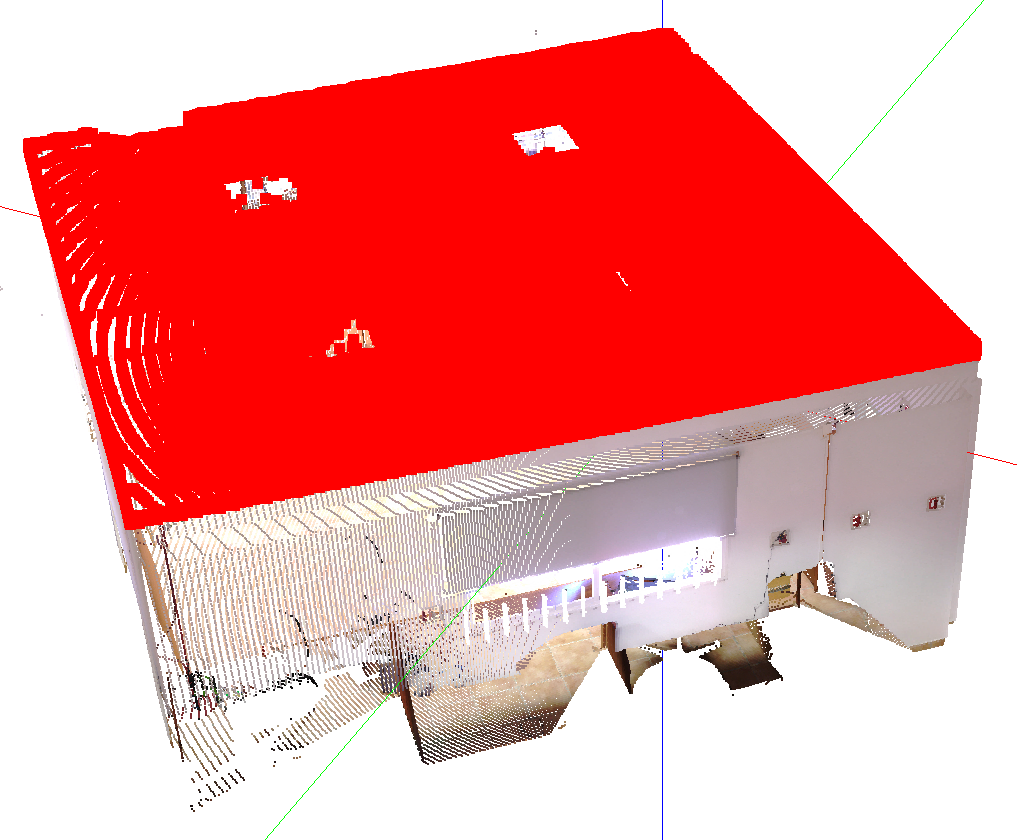
\includegraphics[width=1\linewidth]{lab/lab0-1} 
		%\label{fig:subim1}
	\end{minipage}
	\centering
	\begin{minipage}{0.4\textwidth}
		\centering
		%\includegraphics[width=1\linewidth]{Buyer_call} 
		\includegraphics[width=1\linewidth]{lab/lab0-2} 
		%\label{fig:subim1}
	\end{minipage}
	\begin{minipage}{0.4\textwidth}
		\centering
		%\includegraphics[width=1\linewidth]{Buyer_call} 
		\includegraphics[width=1\linewidth]{lab/lab0-3} 
		%\label{fig:subim1}
	\end{minipage}
	\centering
	\begin{minipage}{0.4\textwidth}
		\centering
		%\includegraphics[width=1\linewidth]{Buyer_call} 
		\includegraphics[width=1\linewidth]{lab/lab0-4} 
		%\label{fig:subim1}
	\end{minipage}
	\begin{minipage}{0.4\textwidth}
		\centering
		%\includegraphics[width=1\linewidth]{Buyer_call} 
		\includegraphics[width=1\linewidth]{lab/lab0-5} 
		%\label{fig:subim1}
	\end{minipage}
	\centering
	\begin{minipage}{0.4\textwidth}
		\centering
		%\includegraphics[width=1\linewidth]{Buyer_call} 
		\includegraphics[width=1\linewidth]{lab/lab0-6} 
		%\label{fig:subim1}
	\end{minipage}
	\caption{De izquierda a derecha y de arriba a abajo los planos que se han ido detectando en la toma 0.}
	\label{fig:planos-lab0}
\end{figure}

\begin{table}[h!]
	\centering
	\begin{tabular}{| c | c | c | c | c |} 
		\hline
		Iteración  & Tiempo (seg.) & Num. puntos \\
		\hline
		1 & 273.455 & 239\,099 \\				  
		2 & 169.57  & 98\,342  \\	
		3 & 113.872 &  27\,342 \\
		4 & 100.32 &   56\,325\\
		5 & 72.0483 & 46\,067 \\
		6 & 64.7628 & 17\,130 \\
		\hline
	\end{tabular}
	\caption{Resultados de aplicar RANSAC en la toma 0 del laboratorio. En la primera columna aparece el número de la iteración, en la segunda el tiempo empleado en segundos y en la tercera el número de puntos que contiene cada plano detectado.}
	\label{table:res-lab0}
\end{table}

\begin{figure}[h!]
		\centering
		%\includegraphics[width=1\linewidth]{Buyer_call} 
		\includegraphics[width=0.6\linewidth]{lab/inter0-pared+mesas} 
		\caption{Intersecciones entre los planos en la toma 0.}
		\label{fig:inter0}
\end{figure}

Repitamos el proceso con la otra toma. Los resultados se encuentras en la figuras \ref{fig:planos-lab1} y \ref{fig:inter1} y en la tabla \ref{table:res-lab1}. \\

\begin{figure}[h!]
	\begin{minipage}{0.5\textwidth}
		\centering
		%\includegraphics[width=1\linewidth]{Buyer_call} 
		\includegraphics[width=1\linewidth]{lab/lab1-1} 
		%\label{fig:subim1}
	\end{minipage}
	\begin{minipage}{0.5\textwidth}
		\centering
		%\includegraphics[width=1\linewidth]{Buyer_call} 
		\includegraphics[width=1\linewidth]{lab/lab1-2} 
		%\label{fig:subim1}
	\end{minipage}
	\begin{minipage}{0.5\textwidth}
		\centering
		%\includegraphics[width=1\linewidth]{Buyer_call} 
		\includegraphics[width=1\linewidth]{lab/lab1-3} 
		%\label{fig:subim1}
	\end{minipage}
	\begin{minipage}{0.5\textwidth}
		\centering
		%\includegraphics[width=1\linewidth]{Buyer_call} 
		\includegraphics[width=1\linewidth]{lab/lab1-4} 
		%\label{fig:subim1}
	\end{minipage}
	\begin{minipage}{0.5\textwidth}
		\centering
		%\includegraphics[width=1\linewidth]{Buyer_call} 
		\includegraphics[width=1\linewidth]{lab/lab1-5} 
		%\label{fig:subim1}
	\end{minipage}
	\begin{minipage}{0.5\textwidth}
		\centering
		%\includegraphics[width=1\linewidth]{Buyer_call} 
		\includegraphics[width=1\linewidth]{lab/lab1-6} 
		%\label{fig:subim1}
	\end{minipage}
	\caption{De izquierda a derecha y de arriba a abajo los planos que se han ido detectando en la toma 1.}
	\label{fig:planos-lab1}
\end{figure}

\begin{table}[h!]
	\centering
	\begin{tabular}{| c | c | c | c | c |} 
		\hline
		Iteración  & Tiempo (seg.) & Num. puntos \\
		\hline
		1 & 342.291 & 269\,194 \\				  
		2 & 203.528  & 103\,483  \\	
		3 & 151.065 &  83\,988 \\
		4 & 90.8403 &  31\,849\\
		5 & 87.0826 & 15\,167 \\
		6 & 75.1206 & 12\,961 \\
		\hline
	\end{tabular}
	\caption{Resultados de aplicar RANSAC en la toma 1 del laboratorio. En la primera columna aparece el número de la iteración, en la segunda el tiempo empleado en segundos y en la tercera el número de puntos que contiene cada plano detectado.}
	\label{table:res-lab1}
\end{table}

\begin{figure}[h!]
	\centering
	%\includegraphics[width=1\linewidth]{Buyer_call} 
	\includegraphics[width=0.6\linewidth]{lab/inter1} 
	\caption{Intersecciones entre los planos en la toma 0.}
	\label{fig:inter1}
\end{figure}

Una vez que hemos obtenido los puntos clave, lo que tenemos que hacer es agruparlos, es decir, ver la correspondencia entre ellos y calcular la transformación que lleva un conjunto en otro. Así, la idea es calcular tres correspondencias y aplicar un prealineado al igual que hicimos en la fase previa del algoritmo ICP. Nuevamente, utilizaremos los descriptores para obtener características significativas de los puntos y poder asignar unos con otros. Para ello, tomamos como referencia el artículo \cite{theiler2012automatic}. En él, propone varios parámetros posibles para formar parte del descriptor aunque el mejor de todos y el que usaremos es el vector formado por los ángulos de intersección de los planos en dicho punto. La explicación de usar este descriptor es que estos ángulos solo dependen de la geometría del modelo y no de otros factores como pueden ser el punto de vista. Una vez los hemos calculado, se obtiene una matriz con las distancias entre los ángulos. Ahora, aplicamos un algoritmo \textit{greedy} o voraz para obtener las tres mejores correspondencias: vamos tomando en cada paso la menor de las distancias siempre y cuando no se repitan puntos ya obtenidos. La razón de que no se puedan repetir los puntos es bastante simple, ya que, de otro modo no se podría realizar el prealineado.  Por ello, el resultado obtenido se muestra en la figura \ref{fig:lab-alineado}. \\

\begin{figure}[h!]
	\centering
	\begin{minipage}{0.6\textwidth}
		\centering
		%\includegraphics[width=1\linewidth]{Buyer_call} 
		\includegraphics[width=1\linewidth]{lab/alineado1} 
		%\label{fig:subim1}
	\end{minipage}
	\centering
	\begin{minipage}{0.6\textwidth}
		\centering
		%\includegraphics[width=1\linewidth]{Buyer_call} 
		\includegraphics[width=1\linewidth]{lab/alineado2} 
		%\label{fig:subim1}
	\end{minipage}
	\caption{Resultado de la alineación.}
	\label{fig:lab-alineado}
\end{figure}

Tal y como se aprecia en la figura, los resultados no han sido los esperados. ¿A qué se puede deber este resultado? En primer lugar, a la propia geometría del modelo. La habitación tiene sus paredes formando un ángulo recto entre ellas lo que hace que todos los descriptores sean bastante parecidos. Sin embargo, como ya hemos dicho: no existe un algoritmo que funcione con todos los modelos. En segundo lugar, a los propios errores de medición a los que se suman los del cálculo de los planos. Esto hace que las pequeñas variaciones que pueda haber se disipen. También tenemos que tener en cuenta las propias apreciaciones realizadas en el articulo tomado como referencia. Indica que la única manera para obtener la solución óptima sería hacer un algoritmo exhaustivo, es decir, probar todas las posibilidades. Ello conllevaría un gasto de tiempo enorme para el cálculo de la alineación al tener que calcular en cada combinación posible la distancia mínima entre los modelos (que ya hemos visto que es muy costoso). Otras posibles soluciones serían, por ejemplo, a partir de esos puntos que el usuario los seleccione manualmente como en el prealineado de ICP. La ventaja frente a esa situación es, que al ser calculados los puntos automáticamente, se obtendría un mejor resultado que si el usuario lo hiciera de una manera visual. Otra opción sería, siempre y cuando se hubiesen obtenido los mismos puntos en ambos casos, calcular la distancia media solo entre los puntos obtenidos mediante RANSAC. \\

También influye en gran medida el número de planos obtenido durante el proceso. Según el artículo de referencia, el porcentaje de acierto con 15 planos no llega ni al 10\% mientras que unos 30 ya ronda el 80\%. Esto hace pensar que el algoritmo será más indicado con modelos más complejos que el usado en nuestro caso.

\section{Ejemplo específico}
En la sección anterior acabamos de ver que el algoritmo propuesto no funcionaba correctamente en nuestro modelo. Como adelantamos, esto no significa que no se pueda utilizar en otras ocasiones en las que podamos disponer de un modelo adecuado. Incluso en \cite{theiler2012automatic}, dice que en el ejemplo que propone no se relizan todas las correspondencias adecuadamente. Por ello, se ha creado un ejemplo \textit{ad hoc} para demostrar que realmente funciona. En nuestro ejemplo ficticio tenemos los planos

\[
\left\{
\begin{array}{rcl}
x &= 2\\ 
y &= 2\\
z &= 2\\
-0.707106x + 0.707106z &= -2
\end{array}
\right.
\]

que conforman una ``toma'. La otra está formada por la rotación de $ \frac{\pi}{2} $ alrededor del eje X, es decir,

\[\\
\left\{
\begin{array}{rcl}
x &= 2\\
z &= 2\\
-y & = 2\\
-0.707106x - 0.707106y &= -2
\end{array}.
\right. 
\]

En la figura \ref{fig:ad-hoc} vemos cómo quedan ambos conjuntos. \\


Los puntos de intersección detectados en el primer conjunto son: $ (2,2,2) $, $ (4.82843,2,2) $ y $ (2,2,-0.82843) $. En el segundo caso, son estos puntos tras aplicar la rotación indicada anteriormente. Los puntos calculados se pueden observar en la figura \ref{fig:ad-hoc2}\\


Si calculamos los ángulos que forman los planos en cada uno de los puntos obtenemos que que en un caso es $ (\frac{\pi}{2}, \frac{\pi}{2}, \frac{\pi}{2}) $, en otro $ (\frac{\pi}{4}, \frac{\pi}{2}, \frac{\pi}{2}) $ y en el último $ (\frac{\pi}{2}, \frac{\pi}{2}, \frac{3\pi}{4}) $. En la otra toma estos valores no varían en los correspondientes puntos. Como vemos, ahora los valores son bastante diferentes entre sí y por ello el algoritmo los asigna correctamente y observamos el resultado en la figura \ref{fig:ad-hoc3}. \\

\begin{figure}[h!]
	\begin{minipage}{0.5\textwidth}
		\centering
		%\includegraphics[width=1\linewidth]{Buyer_call} 
		\includegraphics[width=1\linewidth]{ad-hoc/1} 
		%\label{fig:subim1}
	\end{minipage}
	\begin{minipage}{0.5\textwidth}
		\centering
		%\includegraphics[width=1\linewidth]{Buyer_call} 
		\includegraphics[width=1\linewidth]{ad-hoc/2} 
		%\label{fig:subim1}
	\end{minipage}
	\caption{Planos de ejemplo. Notamos que en una toma se ha modificado la matriz de modelado\footnotemark \hspace{0.5mm}  para poder visualizarlos por separado.}
	\label{fig:ad-hoc}
\end{figure}
\footnotetext{Esta matriz posiciona los puntos en su lugar en coordenadas de mundo.}
\begin{figure}[h!]
	\begin{minipage}{0.5\textwidth}
		\centering
		\includegraphics[width=1\linewidth]{ad-hoc/1-2} 
		%\label{fig:subim1}
	\end{minipage}
	\begin{minipage}{0.5\textwidth}
		\centering
		\includegraphics[width=1\linewidth]{ad-hoc/2-2} 
		%\label{fig:subim1}
	\end{minipage}
	\caption{Puntos de intersección calculados en el ejemplo.}
	\label{fig:ad-hoc2}
\end{figure}

\begin{figure}[bt]
		\centering
		%\includegraphics[width=1\linewidth]{Buyer_call} 
		\includegraphics[width=0.55\linewidth]{ad-hoc/3} 
		%\label{fig:subim1}
	\caption{Resultado de la alineación. Se ha aplicado un leve cambio en una matriz de modelado para poder apreciar la superposición de ambos conjuntos.}
	\label{fig:ad-hoc3}
\end{figure}

Concluimos que los resultados desfavorables obtenidos en la sección anterior se deben sobre todo a la simetría del modelo disponible y que en otros modelos sí es capaz de funcionar correctamente.
%\newpage
%\begin{itemize}
%\item En isprsarchives... : el original parece que es Fishchler and Bolles en 19811.
%\item En isprsarchives... : propone un método mejorado del anterior.
%\item DEcir lo de que es estocástico y cosas de esas.
%\item En theiler... : Puede usarse para el prealineado en ICP 
%\end{itemize}